% Hasentiles! Hase = zajíc (D)

\section{Wang-tile models}

\subsection{Definition}
	
	% Winfree pg 56
	
	We will rather define Wang tile models less formally because it will be clear what they mean and excessive formality could cause confusions.
	
	Wang tile is a square tile with one color (also index, glue) from a finite nonempty set $I$ on each its edge\footnote{Tiles keep orientation, they are {\em not} allowed to rotate nor reflect.}, let us denote (nonempty) set of all available tiles $T$. Wang tiling is a mapping ${\cal T}: (\Z^2) \rightarrow T$ with restrictions: neighboring tiles must have the same color on the adjacent edge and its domain is required to be (topologically) connected. Wang tiling ${\cal T}_2$ is called {\em reachable} from Wang tiling ${\cal T}_1$ iff ${\cal T}_1 \subseteq {\cal T}_2$. A tiling $\cal T$ is called {\em terminal} iff there does not exist any sharply bigger tiling reachable from $\cal T$. %!% říct jaký to uspořádání je, že má minimální prvek
	
	Winfree extends this definition for DNA tile assembly purposes and introduces Abstract Tile Assembly Model (aTAM). Additionally
	\begin{itemize}
		\item every color $c$ is associated with a nonnegative integer $g(c)$ which will also be referred to as {\em glue strength},
		\item there exists an empty color denoted by $\epsilon$ which can be neighboring with arbitrary color,
		\item tiling is only allowed to grow
		\begin{itemize}
			\item from a special initial tile denoted by $t_0$ from $(0,0)$ ({\em initial configuration}),
			\item one tile per step,
			\item the sum of just connected glues must be greater or equal to given integer treshold\footnote{Interesting to study are small numbers like $1$, $2$; there are different results in Section \ref{sec:wang_power}}, so called {\em temperature}, denoted by $\tau$.
		\end{itemize}
	\end{itemize}
	Reachability relation will be restricted accordingly to these rules, {\em reachable in (tilesystem) $T$} will mean reachable from initial configuration, same for {\em terminal tiling in (tilesystem) $T$}.
	
	Similarly to Turing machines, tilesystem $T$ will be called:
	\begin{description}
		\item[Deterministic] iff there exists unique terminal tiling in $T$. % (in other words, reachability relation has one minimal/maximal member).
		\item[Non-deterministic] iff it has no other restrictions. % no ...
		\item[Probabilistic] iff every possible step in every stage has defined probability. See Note \ref{note:tilesystems} for a proposal how the probability could be defined.
	\end{description}
	
	\begin{note}\label{note:tilesystems}
		If there is a unique place and a unique tile the probability is clearly $1$. If there is a unique place but there are more candidate tiles, the probability $\prob_C(t)$ of connecting tile $t$ should be distributed to these tiles somehow according to their concentration ratio (denoted by $\prob_0(t)$) and their total connectible glue strength (denoted by $G(t)$). Most straightforward is weighted average:
		\begin{equation*}
			\prob_C(t) = \frac{G(t)\cdot\prob_0(t)}{\sum\limits_{u\textnormal{ possible tile}}G(u)\cdot\prob_0(u)}
		\end{equation*}
		In the most general case there are more places, each having several candidates. The probability $\prob_C(t,i)$ of connecting tile $t$ on place $i$ can be defined as weighted average again, now with one more sum over all possible places:
		\begin{equation*}
			\prob_C(t,i) = \frac{G(t,i)\cdot\prob_0(t)}{\sum\limits_{j\textnormal{ possible place}}\quad\sum\limits_{u\textnormal{ possible tile}\atop\textnormal{on place }j}G(u,j)\cdot\prob_0(u)}
		\end{equation*}
	\end{note}

\subsection{Computational power}\label{sec:wang_power}
	
	The most exciting thing about aTAM is that
	\begin{itemize}
		\item it is known to be capable of universal computation at temperature $2$ in 2D,
		\item also at temperature $1$ in 3D,
		\item but it is not known to be universal or not at temperature $1$ in 2D\footnote{Universality has been reached only with modifications to the original model, see \cite{stage_assembly}, \cite{active_tiles}.}.
	\end{itemize}
	Let us show known results in a table.
	
	\begin{center}
	\begin{tabular}{|| c || c | c | c ||}
		\hline\hline
		~ & \multicolumn{2}{c|}{\bf $n\times n$ squares} & {\bf Computational} \\
		~ & \multicolumn{1}{c}{LB} & \multicolumn{1}{c|}{UB} & {\bf Power}\\
		\hline
		$\tau=2$, 2D & \multicolumn{2}{c|}{See \cite{square_lb}, $\Theta(\frac{\log n}{\log\log n})$, see \cite{square_ub}} & Universal, see \cite{winfree_phd} \\
		\hline
		$\tau=1$, 3D & $\Omega(\frac{\log n}{\log\log n})$, see \cite{square_lb} & $O(\log n)$, see \cite{cook_temp1} & Universal, see \cite{cook_temp1} \\
		\hline
		$\tau=1$, 2D & $\Omega(\frac{\log n}{\log\log n})$, see \cite{square_lb} & $2n-1$, see \cite{square_lb} & Unknown \\
		\hline\hline
	\end{tabular}
	\end{center}
	
	\subsubsection{Turing universality of 2D tiles at $\tau=2$}
		
		Here we give an alternative and more straightforward 2D tilesystem which directly simulates Turing machine at $\tau=2$ proving Turing universality of this model, see Figures \ref{fig:tileset1} and \ref{fig:tileset2}. Everything is described within these figures. Note that the simulation is deterministic in every step, that the worst case is when changing head's step direction (all the rest must be copied) and thus the slowdown is in $O(t^2(n))$.
		
		\begin{figure}[h]
		\begin{center}
			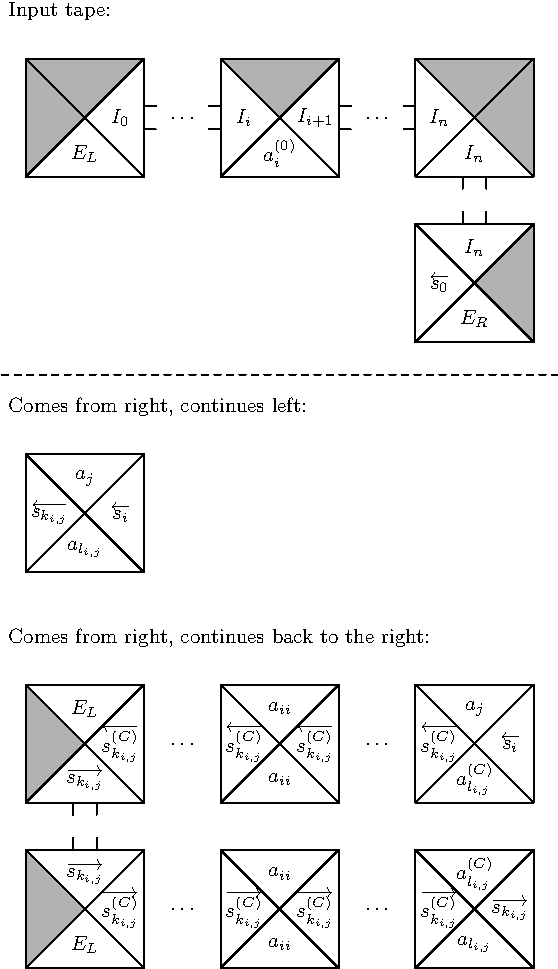
\includegraphics{./figures/tiles1.pdf}
			\caption{Tileset 1/2.}
			\label{fig:tileset1}
		\end{center}
		\end{figure}
		
		\begin{figure}[h]
		\begin{center}
			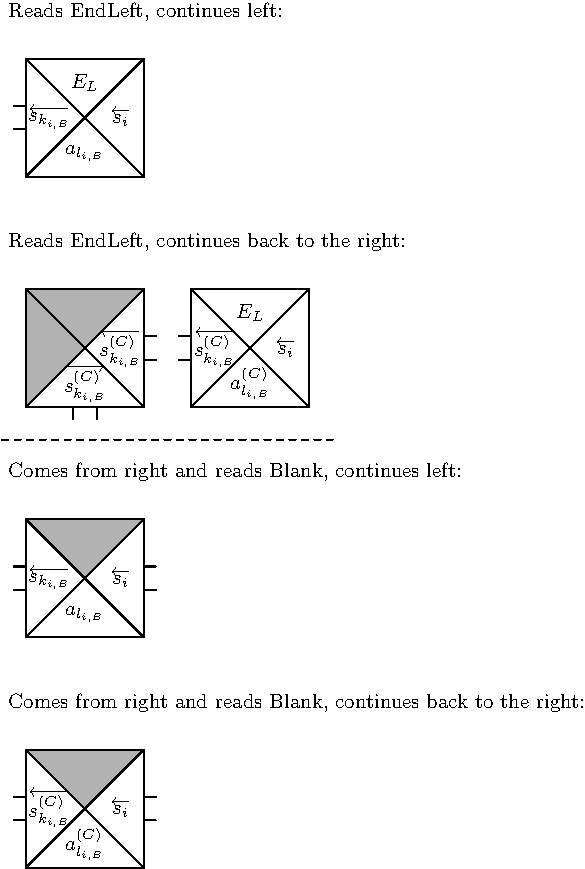
\includegraphics{./figures/tiles2.pdf}
			\caption{Tileset 2/2.}
			\label{fig:tileset2}
		\end{center}
		\end{figure}
	
	%%%%%%%%%%%%%%%%%%%%%%%%%%%%%%%%%%%%%%%%%%%%%%%%%%%%%%%%%%%%%%%%%%%%%%
	
	% error-tolerant rules -- Gacs and Reif, 1988\\
